\chapter{Resultados Preliminares}
\label{cap:res_pre}

Neste capítulo encontram-se os resultados preliminares da primeira e da segunda questão de pesquisa.

\section{QP1. Com que frequência \textit{breaking changes} impactam os clientes}
\label{res:qp1}

\subsubsection{\textbf{10.1\% dos clientes e 8.1\% das \textit{releases} sofreram \textit{breaking changes}}}

Após os clientes/\textit{releases} executarem, os que geraram erros foram analisados para se confirmar a origem do erro: uma chamada à uma função do provedor que contém uma \textit{breaking change} ou alguma alteração realizada pelo cliente. Do total de 184 clientes com erro, 96 sofreram casos de erros internos, enquanto que 45 sofreram algum dos casos particulares de \textit{breaking change}. Por fim, 39 clientes sofreram \textit{breaking changes} em uma de suas \textit{releases}. Também, em 31 clientes houve alguma \textit{release} da qual não foi encontrado o motivo do erro. Porém, um cliente que sofreu uma \textit{breaking change}, por exemplo, pode ter sofrido também com erros internos, e vice-versa, pois um caso não influência na ocorrência dos demais. Por isso, os resultados são melhores apresentados em função das \textit{releases}, uma vez que as \textit{releases} só podem sofrer com apenas um tipo de erro. Dessa maneira, do total de 907 \textit{releases} que sofreram algum erro, foram identificadas 431 \textit{releases} com erros internos, 213 \textit{releases} com erros dos casos particulares de \textit{breaking changes}, 190 erros do caso de \textit{breaking changes} e em 73 \textit{releases} não foi possível descobrir o motivo que gerou o erro. A Figura \ref{fig:pre_res_rq1} contém os resultados em função das \textit{releases}. Assim, os dados sobre os clientes e \textit{releases} que sofreram com \textit{breaking changes} serão utilizados para responder as demais questões de pesquisa.

\begin{figure}
    \centering
    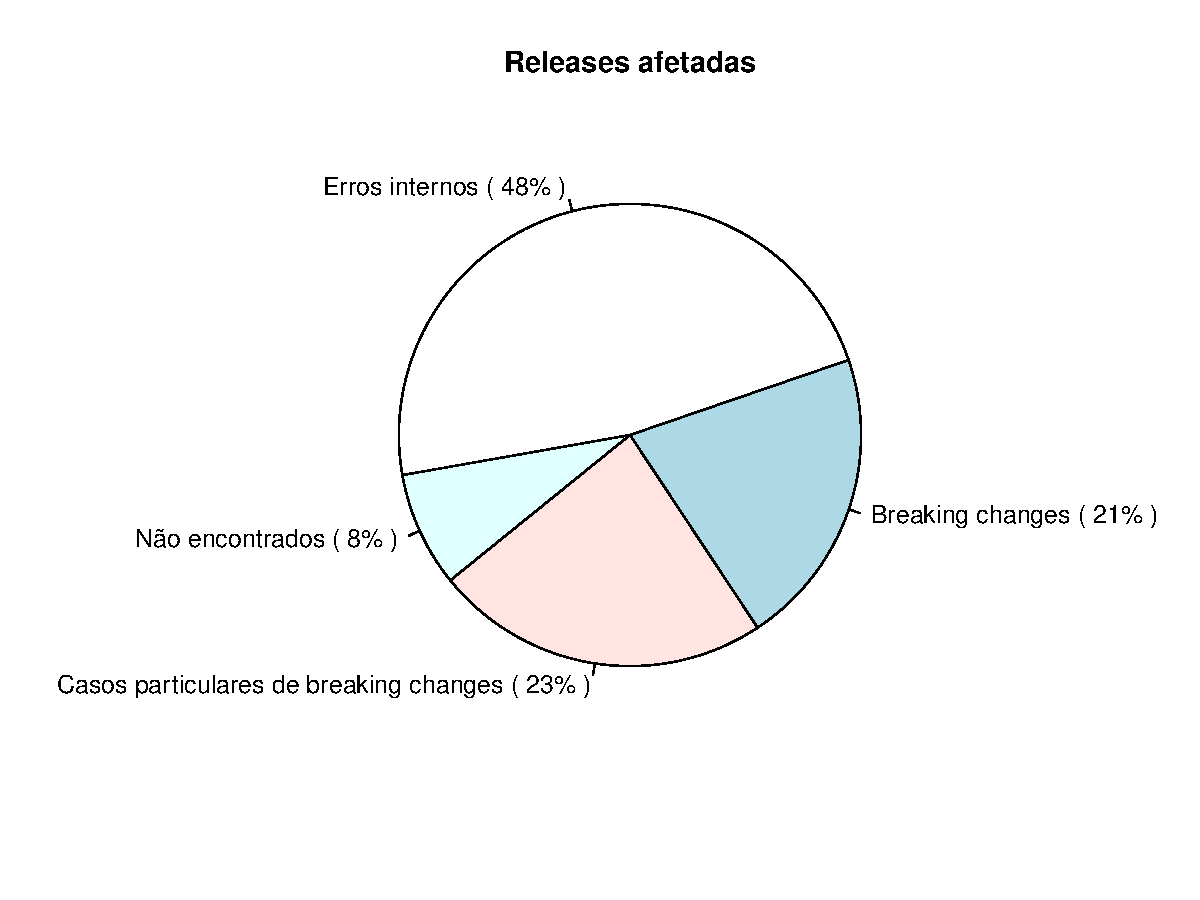
\includegraphics[scale=0.7]{figuras/pre_res_rq1.pdf}
    \caption{Resultado dos casos de erros em função das \textit{releases}}
    \label{fig:pre_res_rq1}
\end{figure}{}

\section{QP2. Como os provedores introduzem \textit{breaking changes} em uma \textit{release}}
\label{res:qp2}

\subsubsection{\textbf{Classificação das \textit{Breaking changes}}}

Ao todo, foram 43 casos de \textit{breaking changes} distribuídas em 39 clientes. Todos esses casos foram agrupados em 8 diferentes categorias das quais se encaixavam. A Tabela \ref{tab:bc_category} apresenta cada uma dessas categorias, bem como a quantidade de clientes e a quantidade de \textit{releases} que cada categoria atingiu.

\begin{table}[]
\begin{tabular}{|l|c|c|c|c|}
\hline
\centering
\textbf{Categoria}           & \textbf{Pacotes afetados} & \textbf{\%}   & \textbf{\textit{Release} afetadas} & \textbf{\%}    \\ \hline
Alteração de regras          & 12              & 27,9 & 64                          & 33,68 \\
Provedores incompatíveis     & 8               & 18,6 & 30                          & 15,78 \\
Alteração de tipo de objeto  & 8               & 18,6 & 24                          & 12,63 \\
Objeto indefinido            & 4               & 9,3  & 25                          & 13,15 \\
Código errado                & 4               & 9,3  & 13                          & 6,84  \\
Código não-atualizado        & 3               & 6,97 & 25                          & 13,15  \\
Renomeação de função         & 3               & 6,97 & 5                           & 2,63  \\
Arquivo não encontrado       & 1               & 2,32 & 4                           & 2,1  \\ \hline
\textbf{Total}               & 43              &      & 190                         &       \\ \hline
\end{tabular}
\caption{Categorias dos casos de \textit{breaking change}}
\label{tab:bc_category}
\end{table}

A seguir, encontra-se uma descrição sobre cada categoria.

\begin{itemize}
    \item \textbf{Alteração de regras}: este caso foi o principal que impactou os clientes. Essa categoria contém os casos de \textit{breaking change} no qual os provedores possuíam um determinado comportamento, mas alteraram algumas de suas regras/funcionalidades e impactaram os seus clientes. Não foi uma simples alteração no código, tal como uma alteração de tipo de variáveis, ou um código escrito de maneira errada, mas sim uma regra no qual o cliente tinha como sólida, foi alterada; %Por exemplo, o pacote \textit{request@2.18.0} introduziu uma alteração em seu código\footnote{https://github.com/request/request/commit/d05b6ba72702c2411b4627d4d89190a5f2aba562\#diff-168726dbe96b3ce427e7fedce31bb0bcR857}, como pode ser visto na Figura \ref{fig:bc_category_change_rule_1}.

    %\begin{figure} \centering 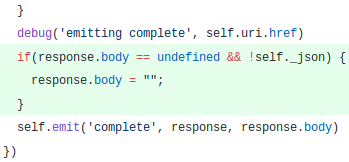
\includegraphics[scale=0.6]{figuras/bc_category_change_rule_1.png} \caption{Alteração de regra de funcionamento do \textit{request}} \label{fig:bc_category_change_rule_1} \end{figure}{}

    %Nesse caso, o \textit{request} adiciona uma \textit{string} vazia ao invés de manter \textit{undefined} o corpo de uma requisição. Esse caso do \textit{request} ocorreu exatamente como foi explicado por \citeonline{Foo:2018:ESC:3236024.3275535} dizendo que os pacotes evoluem independentemente dos clientes. Essa alteração na regra do \textit{request} reflete em uma evolução do pacote, mas o cliente não esperava essa alteração e confiava que o corpo da resposta fosse retornado como \textit{undefined} em caso de erro, por isso o cliente quebrou.

    \item \textbf{Provedores incompatíveis}: nessa categoria, há um provedor direto A e um provedor indireto B envolvido, o qual alterou o seu código, o que não gerou um erro, mas provocou no provedor A um comportamento inesperado, ou seja, o provedor B passou a ser incompatível com o provedor A. Nessa categoria, nenhum dos provedores contém um erro, mas sim uma incompatibilidade; %Um exemplo disso ocorreu com os pacotes \textit{babel-eslint}\footnote{https://www.npmjs.com/package/babel-eslint} e \textit{escope}\footnote{https://www.npmjs.com/package/escope}, entretanto, o pacote \textit{escope} é um provedor indireto do \textit{babel-eslint}.

    %\begin{figure} \centering 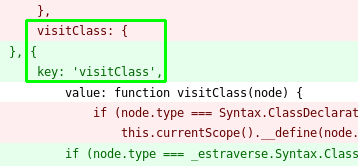
\includegraphics[scale=0.5]{figuras/bc_category_incompatibles_providers.png} \caption{Alteração de código do \textit{escope}} \label{fig:bc_category_incompatibles_providers} \end{figure}{}

    %A \textit{releases escope@3.4} realizou uma alteração no seu código, de acordo com a Figura \ref{fig:bc_category_incompatibles_providers}, mas que não reflete em um erro. Essa alteração impactou diretamente o pacote \textit{babel-eslint}, mesmo o pacote \textit{escope} não sendo um provedor direto do \textit{babel-eslint} e não ter introduzido um erro\footnote{https://github.com/estools/escope/issues/99\#issuecomment-178151491}. Com isso, há uma incompatibilidade entre os provedores e essa incompatibilidade precisou ser corrigida pelo \textit{babel-eslint} e não pelo \textit{escope}. Essa foi a \textit{breaking change} que mais surgiu na análise manual pois, dos 43 casos, 5 (11.6\%) refletiam essa incompatibilidade, uma vez que o \textit{babel-eslint} é provedor de 5.8\% de toda a base de dados.

    \item \textbf{Alteração de tipo de objeto}: essa é uma categoria de \textit{breaking changes} facilmente detectável em linguagens fortemente tipadas, mas no \textit{Javascript} representam um tipo de \textit{breaking change} que, por muitas vezes, pode nem afetar o código do cliente. Mas, neste trabalho, foram detectados 8 (18.6\%) de casos nos quais os provedores alteraram o tipo de alguma variável;

    %\begin{figure} \centering 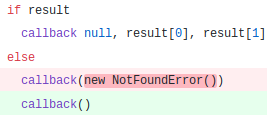
\includegraphics[scale=0.5]{figuras/bc_category_change_type.png} \caption{Alteração de um tipo \textit{array} para \textit{object}} \label{fig:bc_category_change_type} \end{figure}{}

    %Na Figura \ref{fig:bc_category_change_type} o provedor \textit{socket.io}\footnote{https://www.npmjs.com/package/socket.io} alterou alguns \textit{arrays} para \textit{object}\footnote{https://github.com/socketio/socket.io/commit/b73d9bea4efb48277eee685763026ff2df5a79ab}. Anteriormente, os clientes iteravam nesses \textit{arrays}, mas após essa alteração, os clientes foram afetados.

    \item \textbf{Objeto indefinido}: por vezes, os códigos podem estar todos corretos, mas então o provedor tenta acessar uma variável que não existe. Essa categoria de \textit{breaking change} representa os casos no qual os provedores tentaram obter acesso à alguma variável/objeto, mas que não existiam. Esses erros são os que facilmente podem ser consertados/evitados apenas adicionando o código da Listagem \ref{cod:undefined_object}:

    \begin{lstlisting}[style=bash, label=cod:undefined_object]
    this.var = this.var || {};
    \end{lstlisting}

    %Esse tipo de erro surgiu no pacote \textit{ember-cli-htmlbars-inline-precompile}\footnote{https://www.npmjs.com/package/ember-cli-htmlbars-inline-precompile}, no qual o desenvolvedor tenta acessar uma variável que não estava disponível. Mas, assim como o desenvolvedor já havia feito com as demais variáveis da Figura \ref{fig:bc_category_undefined_object}, uma simples alteração no código foi o suficiente.

    %\begin{figure} \centering 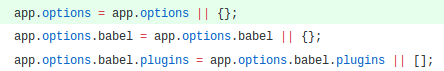
\includegraphics[scale=0.7]{figuras/bc_category_undefined_object.png} \caption{Correção do erro de objeto indefinido} \label{fig:bc_category_undefined_object} \end{figure}{}

    \item \textbf{Código errado}: este caso de \textit{breaking change} ocorreu quando o provedor escreveu um código semanticamente incorreto, gerando um erro na sua execução e afetando o cliente. Em linguagens compilada, esse tipo de erro seria facilmente identificado pelo compilador em tempo de compilação; %Foi exatamente isso que a dependência fez. Ao alterar o seu código, o desenvolvedor escreveu duas vezes a mesma variável, como pode ser visto na Figura \ref{fig:bc_category_wrong_code}. Assim como os erros do tipo \textit{undefined object}, os erros dessa categoria  são facilmente corrigidos.

    %\begin{figure} \centering 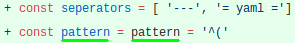
\includegraphics[scale=0.8]{figuras/bc_category_wrong_code.png} \caption{Código semanticamente incorreto} \label{fig:bc_category_wrong_code} \end{figure}{}

    \item \textbf{Código não-atualizado}: as \textit{breaking changes} desta categoria são as que o provedor atualiza o \textit{range} de seu provedor mas não altera o seu código para adaptar-se a ele. Assim, o erro está no primeiro provedor que contém um código desatualizado;

    \item \textbf{Renomeação de função}: as \textit{breaking changes} relacionadas à esta categoria foram facilmente detectáveis. Quando a mensagem de erro do \textit{node.js} era exibida como \textit{TypeError: var is not a function}, com pouca investigação já era possível identificar que uma determinada função não estava mais disponível, ou seja, havia sido removida ou alterado o seu nome; e

    %\begin{figure} \centering 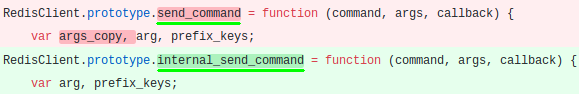
\includegraphics[scale=0.6]{figuras/bc_category_renamed_function.png} \caption{Alteração do nome de função} \label{fig:bc_category_renamed_function} \end{figure}{}

    \item \textbf{Arquivo não encontrado}: os casos de \textit{breaking change} relacionados à esta categoria são aqueles no qual o desenvolvedor realiza um acesso a um arquivo, mas esse não existe. O arquivo requerido pode não existir ou não estar disponível, uma vez que, referenciado no arquivo \textit{.npmignore} -- arquivo utilizado pelo \textit{npm} para ignorar arquivos durante o processo de publicação --, o arquivo existe mas não está disponível, mas também o arquivo pode não existir. Entretanto, o único caso de arquivo não encontrado ocorreu pois o arquivo \textit{index.js} estava referenciado no \textit{.gitignore}.% O provedor \textit{esprima-extract-comments}\footnote{https://www.npmjs.com/package/esprima-extract-comments} utilizava como provedor um \textit{fork} do pacote \textit{esprima}\footnote{https://github.com/ariya/esprima/} e o referencia em seu  \textit{package.json} para ser descarregado diretamente do \textit{Github}\footnote{https://github.com/jonschlinkert/esprima-extract-comments/blob/6b65a0f52f85bc6fa830d44e352ec3da9e9ef620/package.json\#L47}. Entretanto, o \textit{index.js} desse \textit{fork}, foi referenciado no \textit{.gitignore} e não estava disponível quando o \textit{npm} descarregou o pacote diretamente do \textit{Github}, mas o arquivo estava disponível se o pacote \textit{exprima} fosse descarregado diretamente do \textit{npm}.

\end{itemize}{}